\section{Introduction and Background}

\subsection{The Evolving Landscape of Healthcare}
The healthcare industry stands at a critical juncture, grappling with a confluence of persistent challenges that strain its capacity and threaten its sustainability. Escalating operational costs, driven by factors such as an aging global population, the increasing prevalence of chronic diseases, and the high price of advanced medical technologies, place immense pressure on healthcare systems worldwide [1]. Concurrently, healthcare professionals face unprecedented levels of burnout, exacerbated by demanding workloads, administrative burdens, and the emotional toll of patient care [2]. The sheer volume of medical data generated daily—from electronic health records (EHRs), medical imaging, genomic sequencing, and wearable sensors—has surpassed human capacity for manual analysis, creating an information overload that can impede timely and accurate decision-making [3]. Simultaneously, the paradigm is shifting towards personalized medicine, where treatments are tailored to individual patient characteristics, demanding sophisticated analytical capabilities to interpret complex biological and clinical data [4].

Against this backdrop, Artificial Intelligence (AI) has emerged as a transformative force, demonstrating its potential to revolutionize various sectors, including healthcare. AI, broadly defined as the simulation of human intelligence processes by machines, encompasses a range of capabilities such as learning, problem-solving, perception, and decision-making [5]. Early applications in healthcare focused on specific, well-defined tasks, such as image analysis or predictive modeling for disease risk. However, the advent of more sophisticated AI architectures, particularly intelligent agents, promises a more profound impact by enabling systems to perceive their environment, reason about goals, and take autonomous actions to achieve those goals [6]. These agents offer a unique paradigm for addressing the multifaceted and dynamic nature of healthcare challenges, moving beyond static algorithms to dynamic, adaptive systems.

\subsection{Defining AI Agents in Healthcare}
An AI agent is fundamentally a computational entity that perceives its environment through sensors and acts upon that environment through actuators [7]. Key characteristics define an AI agent:
\begin{itemize}
    \item \textbf{Autonomy:} Agents can operate without direct, continuous human intervention, making decisions based on their perceptions and internal states.
    \item \textbf{Goal-Oriented:} Agents are designed with specific objectives or goals they strive to achieve.
    \item \textbf{Adaptability:} Agents can learn from experience and adapt their behavior in response to changes in their environment or new information.
    \item \textbf{Reactivity:} Agents can perceive their environment and respond in a timely fashion to changes that occur in it.
    \item \textbf{Proactiveness:} Agents do not simply act in response to their environment; they exhibit goal-directed behavior by taking initiative.
\end{itemize}
This definition distinguishes AI agents from simpler AI algorithms. While a traditional algorithm might perform a specific calculation (e.g., classifying a medical image), an AI agent could perceive the image, consult patient history, reason about potential diagnoses, recommend a course of action, and even initiate follow-up tasks, all autonomously [8]. In the healthcare context, this translates to systems that can actively assist clinicians, manage patient care pathways, optimize resource allocation, and accelerate research, thereby addressing the complexities that traditional, non-agentic AI approaches struggle to manage. The potential lies in their ability to integrate perception, reasoning, and action within dynamic, real-world healthcare settings.

\subsection{Scope and Objectives of the Article}
This article aims to provide a comprehensive exploration of the current state, diverse applications, inherent challenges, and future trajectory of AI agents within the healthcare domain. We seek to elucidate the fundamental concepts underpinning AI agent technology, examine their practical implementation across various healthcare functions, and critically analyze the ethical, technical, and regulatory hurdles that must be overcome for widespread adoption. Our objective is to offer a balanced perspective, highlighting both the transformative potential and the practical considerations associated with integrating AI agents into the fabric of modern healthcare. The subsequent sections will delve into the core technologies and architectures that enable AI agents, showcase their application in clinical decision support, patient care, administrative tasks, and research, discuss the critical ethical and practical challenges, and finally, project future trends and offer concluding remarks on the responsible advancement of this technology.

\subsection{Article Structure Overview}
The article is structured to guide the reader through a logical progression of topics. Section \ref{sec:concepts} will lay the groundwork by defining key AI agent architectures and the underlying technologies, including a discussion of agent orchestration frameworks like CrewAI. Section \ref{sec:applications} will then explore the diverse applications of AI agents across the healthcare spectrum, from diagnostics and treatment to patient monitoring and drug discovery. Following this, Section \ref{sec:challenges} will critically examine the significant challenges and ethical considerations, including data privacy, bias, trust, and regulatory issues. Finally, Section \ref{sec:future} will look ahead to future trends and conclude with a summary of the key insights and a call for responsible innovation. This structure ensures a thorough understanding of AI agents in healthcare, from foundational principles to future implications.

\section{Core Concepts and Technologies}
\label{sec:concepts}

\subsection{Key AI Agent Architectures}
The design and capabilities of AI agents vary significantly based on their underlying architecture. Understanding these architectures is crucial for appreciating how agents perceive, reason, and act within complex environments like healthcare.

\subsubsection{Reactive Agents}
Reactive agents represent the simplest form of AI agents. They operate based on a direct mapping from percepts to actions, without maintaining an internal state or memory of past experiences beyond what is immediately relevant for the current percept [7]. Their decision-making process is typically a simple lookup table or a set of condition-action rules. For example, a reactive agent monitoring a patient's heart rate might be programmed to trigger an alert if the rate exceeds a predefined threshold. While efficient for simple, immediate responses, reactive agents lack the ability to learn, plan, or exhibit complex goal-directed behavior, limiting their utility in nuanced healthcare scenarios. Their strength lies in their speed and simplicity for tasks requiring immediate, context-independent reactions.

\subsubsection{Deliberative Agents}
Deliberative agents, in contrast, possess internal state, knowledge, and reasoning capabilities that allow them to model the world, plan sequences of actions, and make more informed decisions [9]. These agents maintain a representation of the world, which they update based on incoming percepts. They use this internal model to deliberate on possible actions, considering their potential consequences and how they contribute to achieving their goals. This involves mechanisms for knowledge representation, reasoning, and planning. In healthcare, a deliberative agent could analyze a patient's complete medical history, current symptoms, and diagnostic test results to formulate a treatment plan, considering potential drug interactions and patient comorbidities. This capacity for reasoning and planning makes them far more suitable for complex decision-making tasks than reactive agents.

\subsubsection{Agent Societies / Multi-Agent Systems (MAS)}
Many real-world problems, particularly in healthcare, are too complex for a single agent to solve efficiently. Multi-Agent Systems (MAS) address this by employing a society of interacting agents, each potentially having different capabilities, goals, and knowledge [10]. These agents collaborate, negotiate, and coordinate their actions to achieve individual or collective objectives. In a hospital setting, a MAS could comprise agents responsible for scheduling surgeries, managing bed allocation, coordinating staff, and monitoring patient flow. These agents would need to communicate and negotiate resource availability and task priorities to optimize overall hospital operations. The emergent behavior of the system arises from the interactions among these individual agents, allowing for decentralized problem-solving and increased robustness.

\subsubsection{Hybrid Architectures}
Hybrid agent architectures combine elements of different agent types to leverage their respective strengths. For instance, a hybrid agent might incorporate a reactive layer for immediate responses to critical events (e.g., detecting a sudden drop in blood oxygen levels) while employing deliberative capabilities for longer-term planning and reasoning (e.g., adjusting a ventilator's settings based on a patient's evolving condition over hours) [11]. This approach offers a balance between responsiveness and sophisticated decision-making, making it highly suitable for dynamic and safety-critical environments like healthcare. Frameworks like CrewAI often facilitate the creation of hybrid systems by allowing agents with different specializations and capabilities to work together within a defined crew structure.

\subsection{Underlying AI Technologies}
The development of sophisticated AI agents relies on a suite of interconnected AI technologies that enable perception, learning, reasoning, and interaction.

\subsubsection{Machine Learning (ML) and Deep Learning (DL)}
Machine Learning (ML) algorithms enable agents to learn from data without being explicitly programmed [12]. Deep Learning (DL), a subfield of ML utilizing artificial neural networks with multiple layers, has shown remarkable success in tasks involving complex pattern recognition, such as image analysis, natural language understanding, and prediction. In healthcare, ML/DL models power diagnostic tools that analyze medical images (X-rays, MRIs, CT scans) to detect anomalies [13], predict patient risk scores for various diseases based on historical data, and identify potential drug candidates in pharmaceutical research. Agents use these ML/DL capabilities for perception (interpreting sensor data, recognizing patterns) and for refining their internal models and decision-making strategies based on learned experiences.

\subsubsection{Natural Language Processing (NLP)}
Natural Language Processing (NLP) equips AI agents with the ability to understand, interpret, and generate human language [14]. This is critical for healthcare applications involving textual data, such as clinical notes, research papers, and patient-provider communication. NLP enables agents to extract relevant information from unstructured EHRs, summarize lengthy medical literature, power conversational AI interfaces for patient engagement (chatbots, virtual assistants), and facilitate communication between different healthcare stakeholders. For instance, an agent could process a physician's dictated notes, extract key diagnostic information, and update the patient's structured record automatically.

\subsubsection{Knowledge Representation and Reasoning (KRR)}
Knowledge Representation and Reasoning (KRR) focuses on how to represent information about the world in a form that a computer system can utilize to solve complex problems [15]. This involves creating formalisms (like ontologies, knowledge graphs, or logical rules) to encode medical knowledge, including disease classifications, treatment guidelines, drug interactions, and patient-specific information. Reasoning mechanisms then operate on this represented knowledge to infer new facts, answer queries, and support decision-making. A healthcare agent might use KRR to access and apply clinical practice guidelines, ensuring that its recommendations align with established medical standards.

\subsubsection{Reinforcement Learning (RL)}
Reinforcement Learning (RL) is a type of ML where an agent learns to make a sequence of decisions by trying to maximize a reward signal it receives for its actions in a given environment [16]. The agent explores the environment, takes actions, and receives feedback in the form of rewards or penalties. This trial-and-error process allows the agent to learn optimal policies or strategies over time. In healthcare, RL holds significant promise for optimizing treatment plans for chronic diseases where decisions need to be adapted over long periods, managing dynamic systems like intensive care unit (ICU) ventilators, or personalizing drug dosage adjustments based on real-time patient responses.

\subsection{CrewAI Framework for Agent Orchestration}
CrewAI is an open-source framework designed to simplify the development and deployment of autonomous AI agent teams [1]. It provides a high-level abstraction for orchestrating multiple AI agents, enabling them to collaborate on complex tasks through defined roles, goals, and tool usage.

\subsubsection{Introduction to CrewAI}
CrewAI emphasizes a "role-playing" paradigm where each agent is assigned a specific persona, including a role, backstory, and a set of tools (functions or APIs the agent can use). Agents are organized into "Crews," which are responsible for executing a defined task. The framework manages the delegation of tasks, communication between agents, and the flow of information, allowing developers to focus on defining the agents' capabilities and the overall workflow rather than the intricate details of inter-agent communication and state management [1].

\subsubsection{How CrewAI Facilitates Development}
CrewAI streamlines the development of complex agent systems by:
\begin{itemize}
    \item \textbf{Modularity:} Encouraging the decomposition of complex problems into smaller, manageable tasks, each handled by a specialized agent.
    \item \textbf{Role Specialization:} Enabling the creation of agents with distinct expertise (e.g., research, writing, coding, analysis), mirroring human team structures.
    \item \textbf{Task Delegation:} Automating the process of assigning tasks to the most appropriate agent based on their role and capabilities.
    \item \textbf{Tool Integration:} Providing a flexible mechanism for agents to access and utilize external tools, APIs, and data sources.
    \item \textbf{Simplified Workflow:} Abstracting away much of the underlying complexity of multi-agent coordination, making it easier to build and iterate on agent systems.
\end{itemize}
This approach significantly reduces the development overhead for creating sophisticated AI applications that require collaboration among multiple intelligent entities.

\subsubsection{Illustrative Example of a Healthcare Agent Setup using CrewAI (Conceptual)}
Consider the task of generating a preliminary diagnostic report based on patient symptoms and medical history. Using CrewAI, this could involve:
\begin{itemize}
    \item \textbf{Research Agent:} Tasked with searching medical literature and databases for information related to the patient's reported symptoms and known conditions. Its tools might include web search APIs and access to medical knowledge bases.
    \item \textbf{Analysis Agent:} Tasked with processing the patient's EHR data and the information gathered by the Research Agent. It might use ML models for risk assessment and pattern recognition. Its tools could include data analysis libraries and predictive models.
    \item \textbf{Reporting Agent:} Tasked with synthesizing the findings from the Research and Analysis agents into a coherent draft report. It would leverage NLP capabilities to structure the information logically. Its tools would include text generation models.
    \item \textbf{Clinical Review Agent (Human-in-the-loop):} The final report would be presented to a human clinician for review and approval, ensuring safety and accuracy.
\end{itemize}
The CrewAI framework would orchestrate the flow of information: the Research Agent gathers data, passes it to the Analysis Agent, whose output is then consumed by the Reporting Agent. This structured approach ensures that complex tasks are broken down and handled by specialized agents, leading to a more robust and efficient outcome.

\begin{figure}[htbp]
    \centering
    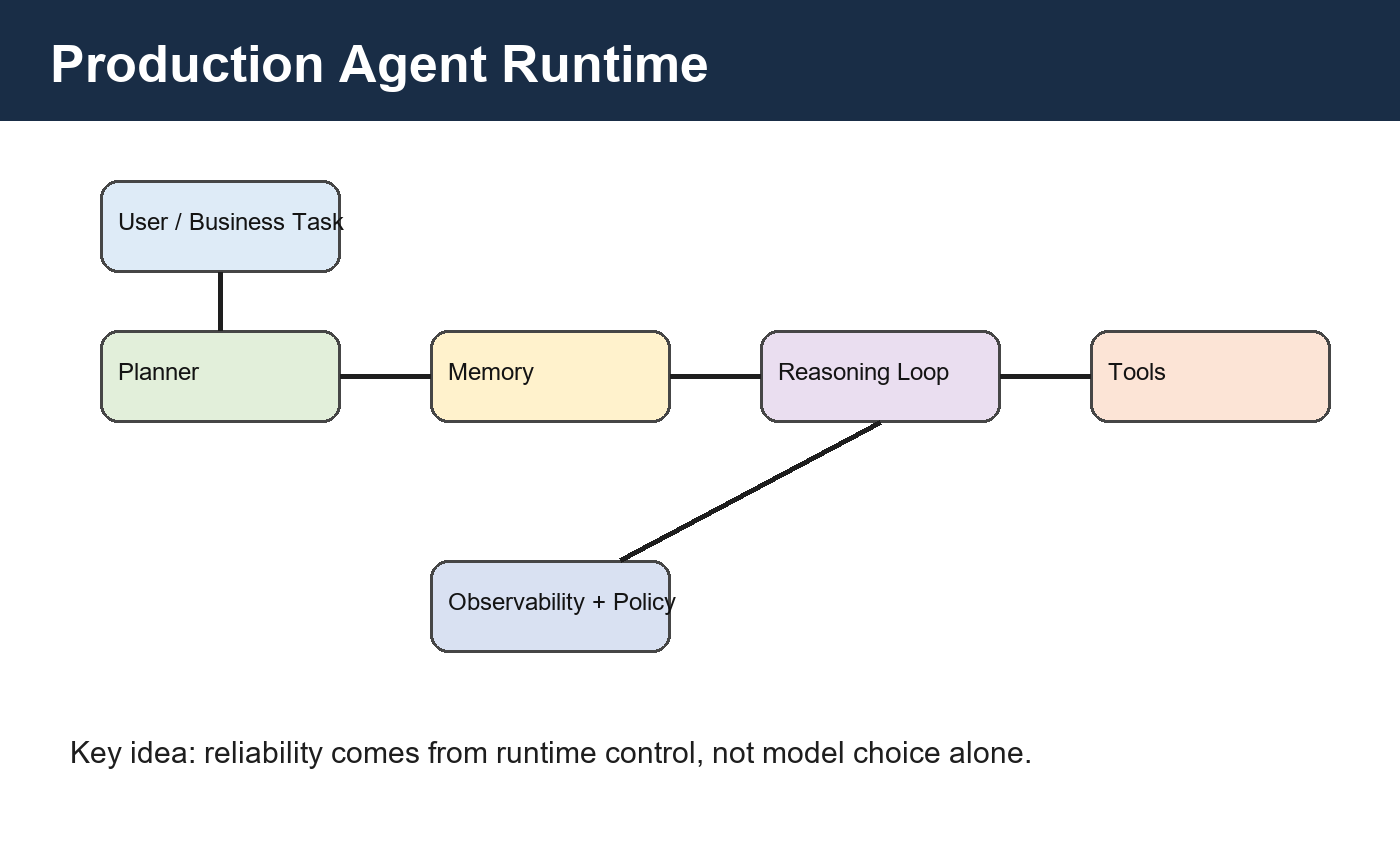
\includegraphics[width=0.8\textwidth]{assets/agent_runtime_architecture.png}
    \caption{Agent Runtime Architecture Overview}
    \label{fig:agent_runtime_architecture}
\end{figure}

\section{Applications of AI Agents in Healthcare}
\label{sec:applications}

\subsection{Clinical Decision Support}
AI agents are poised to revolutionize clinical decision support (CDS) by augmenting the capabilities of healthcare professionals and providing timely, data-driven insights. Traditional CDS systems often rely on predefined rules or statistical models, whereas AI agents can offer more dynamic, context-aware, and personalized support.

\subsubsection{Diagnostic Assistance}
Agents can significantly enhance diagnostic accuracy and speed. By analyzing medical images (radiology, pathology, dermatology) using deep learning models, agents can identify subtle patterns indicative of disease that might be missed by the human eye [13]. For example, an agent could be trained to detect early signs of diabetic retinopathy in retinal scans or identify potentially malignant nodules in lung CT scans. Beyond imaging, agents can process vast amounts of patient data—symptoms, lab results, genetic information, medical history—to suggest differential diagnoses, rank their likelihood, and highlight key supporting or refuting evidence [17]. This is particularly valuable in complex cases with overlapping symptoms or rare diseases. The agent's ability to continuously learn from new cases further refines its diagnostic capabilities over time.

\subsubsection{Treatment Recommendation Systems}
Personalized medicine necessitates treatment plans tailored to individual patient profiles. AI agents can analyze a patient's unique genetic makeup, lifestyle factors, comorbidities, and response to previous treatments to recommend the most effective and least harmful therapeutic options [4]. For instance, in oncology, agents can sift through genomic data to identify specific mutations and match them with targeted therapies or clinical trials [18]. They can also predict a patient's likely response to different drug classes or dosages, considering potential adverse reactions and drug interactions, thereby optimizing treatment efficacy while minimizing side effects. This moves beyond one-size-fits-all approaches to highly individualized care.

\subsubsection{Personalized Medicine and Treatment Planning}
The integration of diverse data streams—genomics, proteomics, metabolomics, EHRs, wearable sensor data—creates a complex picture of individual patient health. AI agents are uniquely suited to synthesize this information for comprehensive treatment planning. They can model disease progression trajectories for individual patients, predict the impact of various interventions, and dynamically adjust treatment plans based on real-time monitoring data [19]. For example, an agent managing a diabetic patient's care could continuously analyze glucose readings, dietary intake, and activity levels to recommend precise insulin dosage adjustments or lifestyle modifications, aiming to maintain optimal glycemic control and prevent long-term complications. This proactive and adaptive approach represents a significant leap forward in personalized healthcare.

\subsection{Patient Care and Monitoring}
AI agents can extend the reach of healthcare services, improve patient engagement, and enable continuous monitoring outside traditional clinical settings.

\subsubsection{Virtual Health Assistants and Chatbots}
Conversational AI agents, powered by NLP, are increasingly used as virtual health assistants and chatbots. These agents can provide patients with 24/7 access to health information, answer frequently asked questions, help schedule appointments, provide medication reminders, and offer support for managing chronic conditions [20]. They can triage patient inquiries, directing urgent cases to human clinicians while handling routine requests autonomously. By engaging patients in a conversational manner, these agents can improve adherence to treatment plans, promote healthier behaviors, and enhance overall patient satisfaction. The ability of these agents to understand natural language and provide empathetic responses is crucial for effective patient interaction.

\subsubsection{Remote Patient Monitoring and Early Detection}
Wearable sensors and home monitoring devices generate continuous streams of physiological data (heart rate, blood pressure, oxygen saturation, activity levels). AI agents can analyze this data in real-time to detect subtle deviations from a patient's baseline or identify early warning signs of health deterioration [21]. For example, an agent monitoring an elderly patient at home could detect changes in gait patterns or sleep disturbances that might indicate an increased risk of falls or the onset of a new health issue, alerting caregivers or clinicians before a critical event occurs. This capability is invaluable for managing chronic diseases, supporting post-operative recovery, and enabling aging-in-place.

\subsubsection{Medication Management and Reminders}
Medication non-adherence is a significant challenge in healthcare, leading to poorer outcomes and increased costs. AI agents can play a crucial role in improving adherence through intelligent reminders, personalized dosing schedules, and checks for potential drug interactions [22]. Smart dispensers integrated with AI agents can ensure patients take the correct medication at the right time and dosage. Agents can also interact with patients to confirm medication intake, answer questions about side effects, and alert clinicians or caregivers if doses are missed, particularly for complex regimens or vulnerable patient populations.

\subsection{Administrative and Operational Efficiency}
Beyond direct clinical applications, AI agents can significantly streamline healthcare operations, reduce administrative burdens, and optimize resource utilization.

\subsubsection{Automating Appointment Scheduling and Resource Allocation}
Hospitals and clinics face complex logistical challenges in managing patient appointments, operating rooms, equipment, and staff schedules. AI agents can automate and optimize these processes. Intelligent scheduling agents can consider patient preferences, physician availability, required resources (e.g., specific surgical equipment), and urgency to create efficient appointment schedules, minimizing wait times and maximizing resource utilization [23]. They can also dynamically reallocate resources in response to unforeseen events, such as emergency admissions or staff absences, ensuring smooth operational flow.

\subsubsection{Streamlining Medical Record Management and Data Entry}
The manual entry and management of medical records are time-consuming and prone to errors. AI agents, particularly those leveraging NLP, can automate significant portions of this workflow. Agents can extract relevant information from dictated notes, scanned documents, or legacy systems and populate structured fields in EHRs [24]. They can also assist in coding medical diagnoses and procedures for billing purposes, ensuring accuracy and compliance. By reducing the data entry burden, agents free up clinical staff to focus more on patient care.

\subsubsection{Fraud Detection and Claims Processing}
The healthcare industry is susceptible to fraud, waste, and abuse in billing and claims. AI agents can analyze vast volumes of claims data to identify anomalous patterns, suspicious billing practices, or potential instances of fraud far more effectively than manual review [25]. By flagging high-risk claims for further investigation, agents help insurers and healthcare providers reduce financial losses and ensure the integrity of the system. Agents can also automate parts of the claims adjudication process, speeding up reimbursement for legitimate claims.

\subsection{Drug Discovery and Development}
The process of discovering and developing new drugs is notoriously long, expensive, and has a high failure rate. AI agents can accelerate multiple stages of this pipeline.

\subsubsection{Accelerating Research through Hypothesis Generation and Simulation}
AI agents can analyze massive datasets from biological experiments, scientific literature, and clinical trials to identify novel correlations and generate testable hypotheses about disease mechanisms or potential drug targets [26]. For example, an agent could analyze gene expression data from healthy and diseased tissues to propose new molecular pathways involved in a disease. Agents can then use simulation environments to predict the efficacy and potential side effects of hypothetical drug compounds *in silico*, significantly reducing the need for costly and time-consuming wet-lab experiments in the early stages of research.

\subsubsection{Identifying Potential Drug Targets and Optimizing Clinical Trial Design}
By processing complex biological data, agents can identify specific proteins, genes, or pathways that are critical to disease progression and thus represent promising targets for therapeutic intervention [18]. Furthermore, AI agents can assist in optimizing clinical trial design by identifying suitable patient cohorts based on specific biomarkers, predicting trial success rates, and even designing adaptive trial protocols that can be modified in real-time based on accumulating data [27]. This leads to more efficient, targeted, and successful clinical trials, ultimately bringing new treatments to patients faster.

\subsection{Surgical Assistance and Robotics}
AI agents are increasingly integrated into surgical environments, enhancing precision, safety, and planning.

\subsubsection{AI-Guided Robotic Surgery}
Robotic surgery systems, enhanced by AI agents, offer surgeons greater precision, dexterity, and visualization. Agents can analyze pre-operative imaging data to create detailed 3D models of the surgical site, identifying critical structures like nerves and blood vessels that must be avoided [28]. During surgery, agents can provide real-time guidance to the robotic instruments, helping the surgeon maintain optimal trajectory, compensate for tremors, and perform minimally invasive procedures with greater accuracy. Some systems may even automate specific sub-tasks under surgeon supervision.

\subsubsection{Pre-operative Planning and Simulation}
Before undertaking complex surgical procedures, AI agents can create highly realistic simulations based on patient-specific anatomy derived from medical scans. Surgeons can use these simulations to rehearse the procedure, anticipate potential complications, and refine their surgical strategy [29]. Agents can analyze variations in anatomy and predict how different surgical approaches might play out, allowing for meticulous planning that minimizes risks and improves patient outcomes. This virtual rehearsal environment is invaluable for training surgeons and preparing for challenging operations.

\section{Challenges and Ethical Considerations}
\label{sec:challenges}

\subsection{Data Privacy and Security}
The use of AI agents in healthcare inherently involves the processing of vast amounts of sensitive patient data, raising significant concerns regarding privacy and security. Protecting this data is paramount, both ethically and legally.

\subsubsection{Handling Sensitive Patient Data}
Healthcare data, including Electronic Health Records (EHRs), diagnostic images, and genomic information, is highly personal and confidential. Regulations such as the Health Insurance Portability and Accountability Act (HIPAA) in the United States and the General Data Protection Regulation (GDPR) in Europe impose strict requirements on how this data can be collected, stored, processed, and shared [30, 31]. AI agents must be designed and implemented in strict compliance with these regulations. This involves robust data anonymization and de-identification techniques, secure data storage, access control mechanisms, and transparent data usage policies. Ensuring that agents do not inadvertently expose or misuse patient information is a critical design challenge.

\subsubsection{Cybersecurity Risks}
AI systems, like any software, are vulnerable to cyberattacks. In the healthcare context, a successful attack on an AI agent system could have severe consequences, ranging from data breaches and theft of sensitive information to disruption of critical healthcare services or even direct harm to patients if diagnostic or treatment agents are compromised [32]. Malicious actors could attempt to manipulate agent algorithms, inject false data, or exploit vulnerabilities in the agent's communication channels or underlying infrastructure. Therefore, comprehensive cybersecurity measures, including regular security audits, intrusion detection systems, secure coding practices, and robust authentication protocols, are essential for protecting AI agent deployments in healthcare.

\subsection{Bias and Fairness}
AI algorithms learn from data, and if the training data reflects existing societal biases, the resulting AI systems can perpetuate or even amplify these inequities. This is a particularly acute concern in healthcare, where biased algorithms can lead to disparities in diagnosis, treatment, and health outcomes.

\subsubsection{Algorithmic Bias in Training Data}
Historical healthcare data may contain biases related to race, gender, socioeconomic status, or geographic location. For example, if a diagnostic algorithm is trained predominantly on data from a specific demographic group, it may perform poorly or inaccurately when applied to patients from underrepresented groups [33]. Similarly, biases in clinical trial data can lead to treatments that are less effective for certain populations. AI agents trained on such data risk making biased recommendations, leading to inequitable care.

\subsubsection{Ensuring Fairness and Equity in AI-Driven Healthcare}
Addressing algorithmic bias requires a multi-pronged approach. This includes curating diverse and representative training datasets, developing bias detection and mitigation techniques within AI algorithms [34], and implementing fairness metrics to continuously monitor agent performance across different demographic groups. Transparency in how agents make decisions and the data they rely on is also crucial. Furthermore, ongoing audits and regulatory oversight are necessary to ensure that AI agents contribute to reducing, rather than exacerbating, health disparities and promote equitable access to quality care for all individuals.

\subsection{Explainability and Trust}
The complexity of many AI models, particularly deep learning systems, often results in a lack of transparency, commonly referred to as the "black box" problem. This lack of understanding can hinder trust and adoption among healthcare professionals and patients.

\subsubsection{The "Black Box" Problem}
Many advanced AI algorithms, such as deep neural networks, operate in ways that are not easily interpretable by humans. It can be difficult to understand precisely why an agent arrived at a particular diagnosis or treatment recommendation [35]. This opacity is problematic in healthcare, where clinicians need to understand the rationale behind decisions to validate them, take responsibility, and explain them to patients. Without explainability, clinicians may be hesitant to rely on AI recommendations, especially in high-stakes situations.

\subsubsection{Building Trust Among Clinicians and Patients}
Establishing trust requires AI agents to be not only accurate but also understandable and reliable. Techniques in Explainable AI (XAI) aim to provide insights into the decision-making process of AI systems [36]. This might involve highlighting the key features or data points that influenced an agent's conclusion, providing confidence scores, or generating natural language explanations. Furthermore, rigorous validation, transparent reporting of performance metrics and limitations, and demonstrating consistent, safe operation over time are essential for building trust. Patient education about how AI agents are used in their care is also vital for fostering acceptance.

\subsection{Regulatory and Legal Frameworks}
The rapid advancement of AI technology often outpaces the development of appropriate regulatory and legal frameworks, creating uncertainty and challenges for the deployment of AI agents in healthcare.

\subsubsection{Navigating the Evolving Regulatory Landscape}
Regulatory bodies worldwide are grappling with how to oversee AI-driven medical devices and software. Frameworks are needed to ensure the safety, efficacy, and ethical use of AI agents in clinical settings [37]. This includes establishing clear guidelines for the development, validation, approval, and post-market surveillance of AI-based healthcare tools. The dynamic nature of AI, particularly its ability to learn and adapt, poses unique challenges for traditional regulatory models that are often based on static product approvals.

\subsubsection{Liability and Accountability}
Determining liability when an AI agent makes an error that leads to patient harm is a complex legal question. Is the developer, the deploying institution, the clinician who relied on the agent, or the agent itself (if considered sufficiently autonomous) responsible? Clear legal frameworks are needed to assign accountability and provide recourse for patients who may be affected by AI-related errors [38]. This requires careful consideration of the agent's autonomy, the level of human oversight, and the contractual agreements between technology providers and healthcare institutions.

\subsection{Integration with Existing Healthcare Systems}
The integration of new AI agent technologies into the complex and often fragmented landscape of existing healthcare IT infrastructure presents significant technical and organizational hurdles.

\subsubsection{Interoperability Challenges}
Healthcare systems typically comprise a diverse array of legacy IT systems, EHR platforms, imaging archives (PACS), and laboratory information systems. Achieving seamless interoperability—the ability of these disparate systems and the AI agents to exchange and interpret data effectively—is a major challenge [39]. Lack of standardized data formats and communication protocols can impede the flow of information necessary for AI agents to function optimally. Significant investment in middleware, data harmonization efforts, and adherence to interoperability standards (like HL7 FHIR) is required.

\subsubsection{Resistance to Adoption}
Beyond technical integration, organizational and cultural factors can influence the adoption of AI agents. Healthcare professionals may be resistant due to concerns about job security, skepticism about the technology's reliability, lack of adequate training, or disruption to established workflows [40]. Overcoming this resistance requires effective change management strategies, including demonstrating the value proposition of AI agents, providing comprehensive training and support, involving clinicians in the design and implementation process, and fostering a culture that embraces innovation.

\subsection{The Human Element}
Despite the increasing sophistication of AI agents, the human element remains central to healthcare. Striking the right balance between AI capabilities and human judgment is crucial for maintaining high-quality, patient-centered care.

\subsubsection{Maintaining the Doctor-Patient Relationship}
The core of healthcare lies in the relationship between the clinician and the patient, built on empathy, trust, and communication. Over-reliance on AI agents could potentially depersonalize care or reduce the time clinicians spend engaging directly with patients [41]. It is essential that AI agents are designed as tools to augment, rather than replace, human interaction, freeing up clinicians to focus on the aspects of care that require human connection and nuanced understanding.

\subsubsection{The Role of Human Oversight and Judgment}
While AI agents can process data and identify patterns with remarkable speed and accuracy, human clinicians bring critical judgment, ethical reasoning, and contextual understanding that AI currently lacks. Complex or ambiguous cases, ethical dilemmas, and situations requiring deep empathy often necessitate human intervention and final decision-making [42]. Maintaining appropriate levels of human oversight ensures that AI-driven recommendations are critically evaluated within the broader context of the patient's well-being and individual circumstances, safeguarding against potential AI errors or biases.

\section{Future Trends and Conclusion}
\label{sec:future}

\subsection{Advanced Agent Capabilities}
The evolution of AI agents in healthcare is moving towards more sophisticated, proactive, and privacy-preserving capabilities, promising a future where AI is deeply integrated into the healthcare ecosystem.

\subsubsection{Proactive and Predictive Healthcare}
Future AI agents will likely shift from reactive support to proactive and predictive healthcare. By continuously analyzing longitudinal patient data from various sources (EHRs, wearables, genomics, social determinants of health), agents will be able to anticipate health risks long before symptoms manifest [19]. This will enable timely interventions, personalized preventative strategies, and a transition from disease treatment to health maintenance. Agents could predict disease outbreaks within communities or identify individuals at high risk for specific conditions, allowing for targeted public health initiatives and personalized wellness plans.

\subsubsection{Federated Learning for Privacy-Preserving AI}
Federated learning offers a promising approach to train AI models, including those used by healthcare agents, without centralizing sensitive patient data [43]. In this paradigm, models are trained locally on data residing within individual healthcare institutions or devices. Only the model updates (parameters or gradients), not the raw data, are shared and aggregated to create a global model. This significantly enhances data privacy and security, making it feasible to develop powerful AI agents trained on diverse datasets while respecting patient confidentiality and regulatory requirements like HIPAA and GDPR.

\subsubsection{Explainable AI (XAI) Advancements}
The demand for trust and transparency will continue to drive advancements in Explainable AI (XAI). Future XAI techniques will likely provide more intuitive and clinically relevant explanations for AI agent decisions [36]. This could involve generating counterfactual explanations ("what would need to change for the diagnosis to be different?"), causal reasoning to understand the underlying mechanisms, or interactive visualization tools that allow clinicians to explore the agent's reasoning process. Enhanced explainability will be crucial for regulatory approval, clinical adoption, and building confidence among both providers and patients.

\subsection{The Role of AI Agents in a Pandemic/Public Health Crisis}
The COVID-19 pandemic highlighted the critical need for agile and intelligent systems to manage public health emergencies. AI agents are well-suited to play a vital role in future crises.

\subsubsection{Rapid Response, Resource Management, and Information Dissemination}
During a pandemic, AI agents can rapidly analyze epidemiological data to model disease spread, predict resource needs (e.g., hospital beds, ventilators, vaccines), and optimize supply chain logistics [44]. They can power intelligent chatbots to provide accurate public health information, combat misinformation, and assist with contact tracing. Agents can also help manage healthcare workforce allocation, identify emerging treatment protocols based on real-time clinical data, and accelerate the analysis of research findings to inform public health policy. Their ability to process vast amounts of data quickly and coordinate complex responses makes them invaluable assets in crisis management.

\subsection{Towards Autonomous Healthcare Systems}
The long-term vision for AI in healthcare involves increasingly autonomous systems that can manage significant aspects of patient care and operations with minimal human intervention, while always maintaining appropriate human oversight for critical decisions.

\subsubsection{Vision for the Future of AI-Integrated Healthcare}
Imagine a future where AI agents continuously monitor population health trends, proactively identify individuals at risk, deliver personalized preventative interventions, manage chronic conditions with adaptive treatment plans, and optimize hospital operations seamlessly. These agents would act as intelligent collaborators for clinicians, handling routine tasks, providing deep analytical insights, and enabling a shift towards a more preventative, personalized, and efficient healthcare model [45]. This vision requires not only technological advancement but also careful consideration of ethical implications, regulatory frameworks, and the integration of human judgment. The goal is not to replace human caregivers but to empower them with advanced tools that enhance their capabilities and improve patient outcomes.

\subsection{Concluding Remarks}
\subsubsection{Summary of Key Findings}
This article has explored the multifaceted role of AI agents in healthcare, from their foundational concepts and underlying technologies to their diverse applications and the significant challenges they present. We have examined how frameworks like CrewAI facilitate the orchestration of specialized agents, enabling complex tasks in areas such as clinical decision support, patient monitoring, administrative efficiency, and drug discovery. The potential for AI agents to enhance diagnostic accuracy, personalize treatments, improve operational efficiency, and accelerate research is immense. However, realizing this potential requires addressing critical issues related to data privacy, algorithmic bias, explainability, regulatory hurdles, system integration, and the indispensable role of human oversight.

\subsubsection{Reiteration of the Transformative Potential}
AI agents represent a paradigm shift in how healthcare can be delivered and managed. By moving beyond static algorithms to dynamic, autonomous, and collaborative systems, they offer unprecedented opportunities to tackle the persistent challenges facing the healthcare industry. Their ability to learn, adapt, and act upon complex data holds the promise of making healthcare more precise, accessible, efficient, and ultimately, more effective for patients worldwide. The integration of advanced AI capabilities, coupled with robust governance and ethical considerations, will pave the way for a future where healthcare is more proactive, personalized, and data-driven.

\subsubsection{Call to Action for Responsible Development and Deployment}
The journey towards widespread adoption of AI agents in healthcare must be guided by a commitment to responsible innovation. This necessitates collaboration among researchers, developers, clinicians, policymakers, and patients to ensure that these powerful technologies are developed and deployed in a manner that is safe, ethical, equitable, and beneficial to all. Continuous research into areas like XAI, federated learning, and bias mitigation, coupled with the establishment of clear regulatory pathways and robust cybersecurity measures, will be essential. Ultimately, the successful integration of AI agents hinges on a shared vision that prioritizes patient well-being, enhances clinical practice, and fosters a healthcare system that is both technologically advanced and deeply human.

\begin{figure}[htbp]
    \centering
    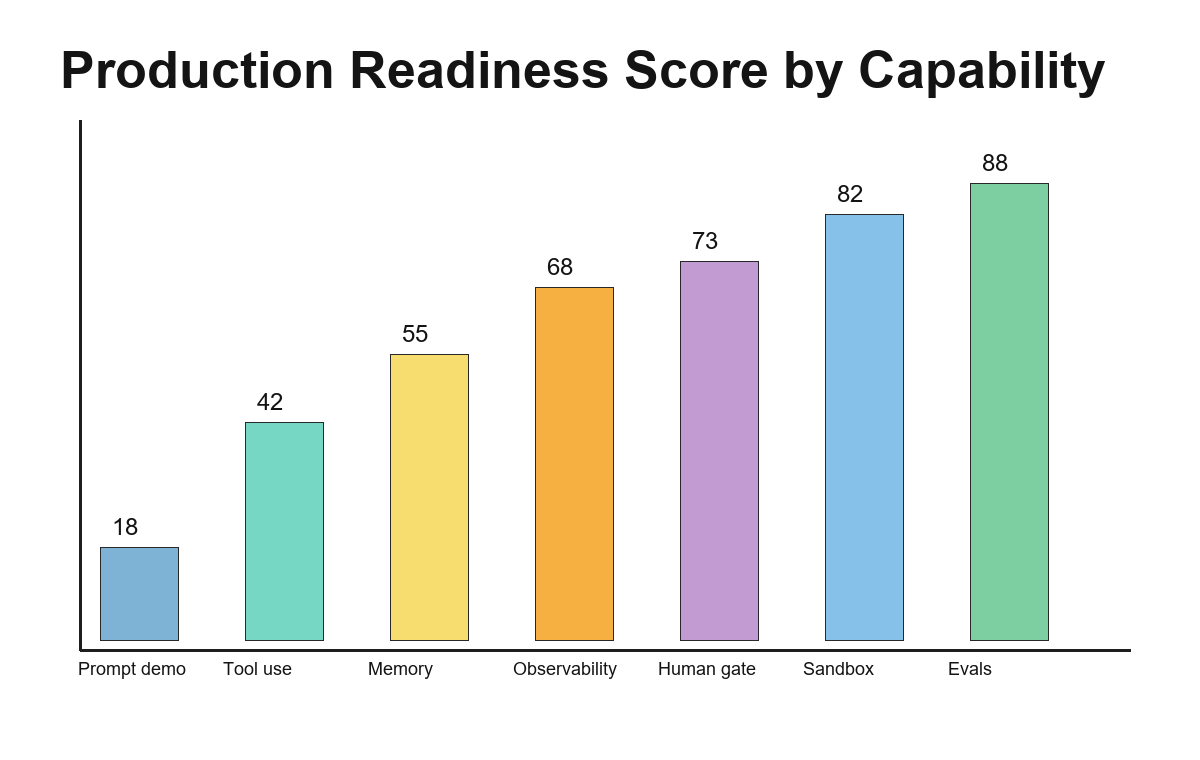
\includegraphics[width=0.8\textwidth]{assets/readiness_chart.png}
    \caption{AI Agent Readiness Assessment Chart}
    \label{fig:readiness_chart}
\end{figure}

\begin{table}[htbp]
    \centering
    \caption{Comparison of AI Agent Architectures}
    \label{tab:agent_architectures}
    \begin{tabular}{@{}lll@{}}
        \toprule
        Feature & Reactive Agents & Deliberative Agents \\
        \midrule
        Internal State & None & Yes \\
        Learning Capability & Limited/None & Yes \\
        Planning & No & Yes \\
        Response Time & Fast & Slower (due to deliberation) \\
        Complexity Handling & Low & High \\
        Healthcare Example & Simple alert system & Treatment planning \\
        \bottomrule
    \end{tabular}
\end{table}

The readiness equation for AI agent deployment can be conceptualized as:
\begin{equation}
    R = \frac{C \times T \times E}{U}
    \label{eq:readiness}
\end{equation}
where $R$ is the overall readiness score, $C$ represents the technological capability of the agent, $T$ signifies the trustworthiness and reliability of the system, $E$ denotes the ethical and regulatory compliance, and $U$ is the user (clinician/patient) adoption and understanding. A high readiness score indicates that an AI agent is well-prepared for deployment in a healthcare setting.

\section{Bilingual BiDi Demonstration}
\begin{hebrew}
\begin{flushright}
עמוד זה מדגים שילוב אמיתי של עברית ואנגלית בתוך מסמך LaTeX. הטקסט מיושר לימין ונשמר כטקסט חי, לא כתמונה.
\end{flushright}
\end{hebrew}
